\documentclass[a4paper]{article}

%% Language and font encodings
\usepackage[german]{babel}
\usepackage[utf8x]{inputenc}
\usepackage[T1]{fontenc}
\usepackage{caption}
\usepackage{wrapfig}

%% Sets page size and margins
\usepackage[a4paper,top=3cm,bottom=2cm,left=3cm,right=3cm,marginparwidth=1.75cm]{geometry}

%% Useful packages
\usepackage{amsmath}
\usepackage{graphicx}
\usepackage[colorinlistoftodos]{todonotes}
\usepackage[colorlinks=true, allcolors=black]{hyperref}
\usepackage{setspace}
\usepackage{listings}

\title{Bankomat mittels Boost.[SML]}
\author{von Jakob Wildt}

\begin{document}

\maketitle
\large

\begin{center}
\end{center}
\newpage
\begin{spacing}{1,5}


\newpage
\section{Eidesstaatliche Erklärung}

Hiermit erkläre ich an Eides statt, dass ich die vorliegende Arbeit selbstständig und ohne fremde Hilfe verfasst und keine anderen als die im Literaturverzeichnis angegebenen Quellen und Hilfsmittel verwendet habe. Insbesondere versichere ich, dass ich alle wörtlichen und sinngemäßen Übernahmen aus anderen Werken als solche kenntlich gemacht habe.
\newline
\newline
\newline
\newline
\newline
\newline
---------------------------------------------------------------------------------------------------------------------------------
\newline
Ort, Datum
\hspace{300pt}
Unterschrift

\newpage

\tableofcontents

\newpage

\section{Einleitung}

Die folgende Dokumentation beschreibt das Projekt "Bankomat [Boost].SML". Es handelt sich um ein Schulprojekt, das durchgeführt wurde um eine Note zu verbessern. \newline
Es handelt sich um einen Automaten, der über die Kommandozeile bedient werden kann und auf Basis eines österreichischen Bankomaten implementiert wurde.  

\newpage

\section{[Boost].SML}

[Boost].SML, die "Weiterentwicklung" von Boost.MSM ist eine header-only State Machine Library. Die Bibliothek dient zur Vereinfachung und Strukturierung von komplizierten State Machine-Code in C++ und kann ab dem C-Standard 2014 verwendet werden.

\subsection{Installation}

Die Library kann unter dem Link: https://boost-experimental.github.io/sml/index.html heruntergeladen werden. Daraufhin muss sie nur mehr mithilfe eines include-Befehls eingebunden werden.
\begin{lstlisting}[language=c++]
#include "boost/sml.hpp"
\end{lstlisting}

\subsection{Funktionen}

\subsubsection{States}

Die Zustände eines Automaten werden durch States beschrieben. In [Boost].SML müssen die Zustände nicht unbedingt im Vorhinein definiert werden. Eine Definition im Transition Table reicht aus, dazu später mehr.

\subsubsection{Events}

Events führen Zustandsübergänge herbei und müssen im Gegensatz zu den Zuständen definiert werden, bevor sie im Transition Table verwendet werden können. Sie können als Instanz angelegt werden \begin{lstlisting}[language=c++]
auto event = sml::event<my_event>;
\end{lstlisting} oder als neuer Datentyp implementiert werden.
\begin{lstlisting}[language=c++]
struct my_event { ... };
\end{lstlisting}

\newpage

\subsubsection{Guards und Actions}

Guards und Actions sind Objekte, die von der State Machine verarbeitet werden, um zu überprüfen ob ein Zustandsübergang (manchmal gefolgt von einer Aktion) durchgeführt werden soll. Guards returnen immer einen boolschen Wert, während Actions nicht zwingend etwas zurückgeben müssen.
\newline\newline
Beispiele für die Implementierung von Guards wären:

\begin{lstlisting}[language=c++]
auto guard1 = [] {
  return true;
};

auto guard2 = [](int, double) { // guard with dependencies
  return true;
};

const auto right_PIN = [](PIN& pin, Karte& karte){
    std::cout << "PIN VALUE: " << pin.value << std::endl;
    return pin.value == karte.pin;
};
\end{lstlisting}
Actions wurden in diesem Projekt nicht verwendet, hier sind jedoch die Beispiele des offiziellen [Boost].SML Tutorials:

\begin{lstlisting}[language=c++]
auto action1 = [] { };
auto action2 = [](int, double) { }; // action with dependencies
auto action3 = [](int, auto event, double) { }; // action with an event and dependencies
struct action4 {
    void operator()() noexcept { }
};
\end{lstlisting}

\newpage

\subsubsection{State Machine und Transition Table}

Um eine State Machine zu erstellen, braucht man immer einen Transition Table - also eine Zustandsübergangstabelle. Sie beschreibt in welchen Zustand welcher Input welchen Zustandsübergang bewirkt. Der Automat wird als eigene Klasse definiert und eine Instanz davon dann ausgeführt.

\begin{lstlisting}[language=c++]
namespace sml = boost::sml;

namespace {
struct e1 {};
struct e2 {};
struct e3 {};

struct transitions {
  auto operator()() const noexcept {
    using namespace sml;
    return make_transition_table(
       *"idle"_s                  / []
       { std::cout << "anonymous transition" << std::endl; } = "s1"_s
      , "s1"_s + event<e1>        / []
      { std::cout << "internal transition" << std::endl; }
      , "s1"_s + event<e2>        / []
      { std::cout << "self transition" << std::endl; } = "s1"_s
      , "s1"_s + sml::on_entry<_> / []
      { std::cout << "s1 entry" << std::endl; }
      , "s1"_s + sml::on_exit<_>  / []
      { std::cout << "s1 exit" << std::endl; }
      , "s1"_s + event<e3>        / []
      { std::cout << "external transition" << std::endl; } = X
    );
  }
};
}  

int main() {
  sml::sm<transitions> sm;
  sm.process_event(e1{});
  sm.process_event(e2{});
  sm.process_event(e3{});
  assert(sm.is(sml::X));
}
\end{lstlisting}

\newpage

\section{Bankomat}

Im folgenden Abschnitt wird die Funktionsweise sowie die Bedienung des Bankomaten genauer erklärt. 

\subsection{UML-Diagramm}

Das UML-Diagramm soll den Ablauf veranschaulichen und alle möglichen Zustandsänderungen anzeigen. Die Rechtecke beschreiben die Zustände und die Kanten die Zustandsübergänge. Zustandsübergänge sind oft mit aktion1/aktion2 beschriftet, wobei ''aktion1'' für die Eingabe steht, die den Zustandsübergang zur Folge hat und ''aktion2'' für die mögliche Ausgabe, die aus dem Zustandswechsel folgt.


\begin{figure}[h!]
\begin{center}
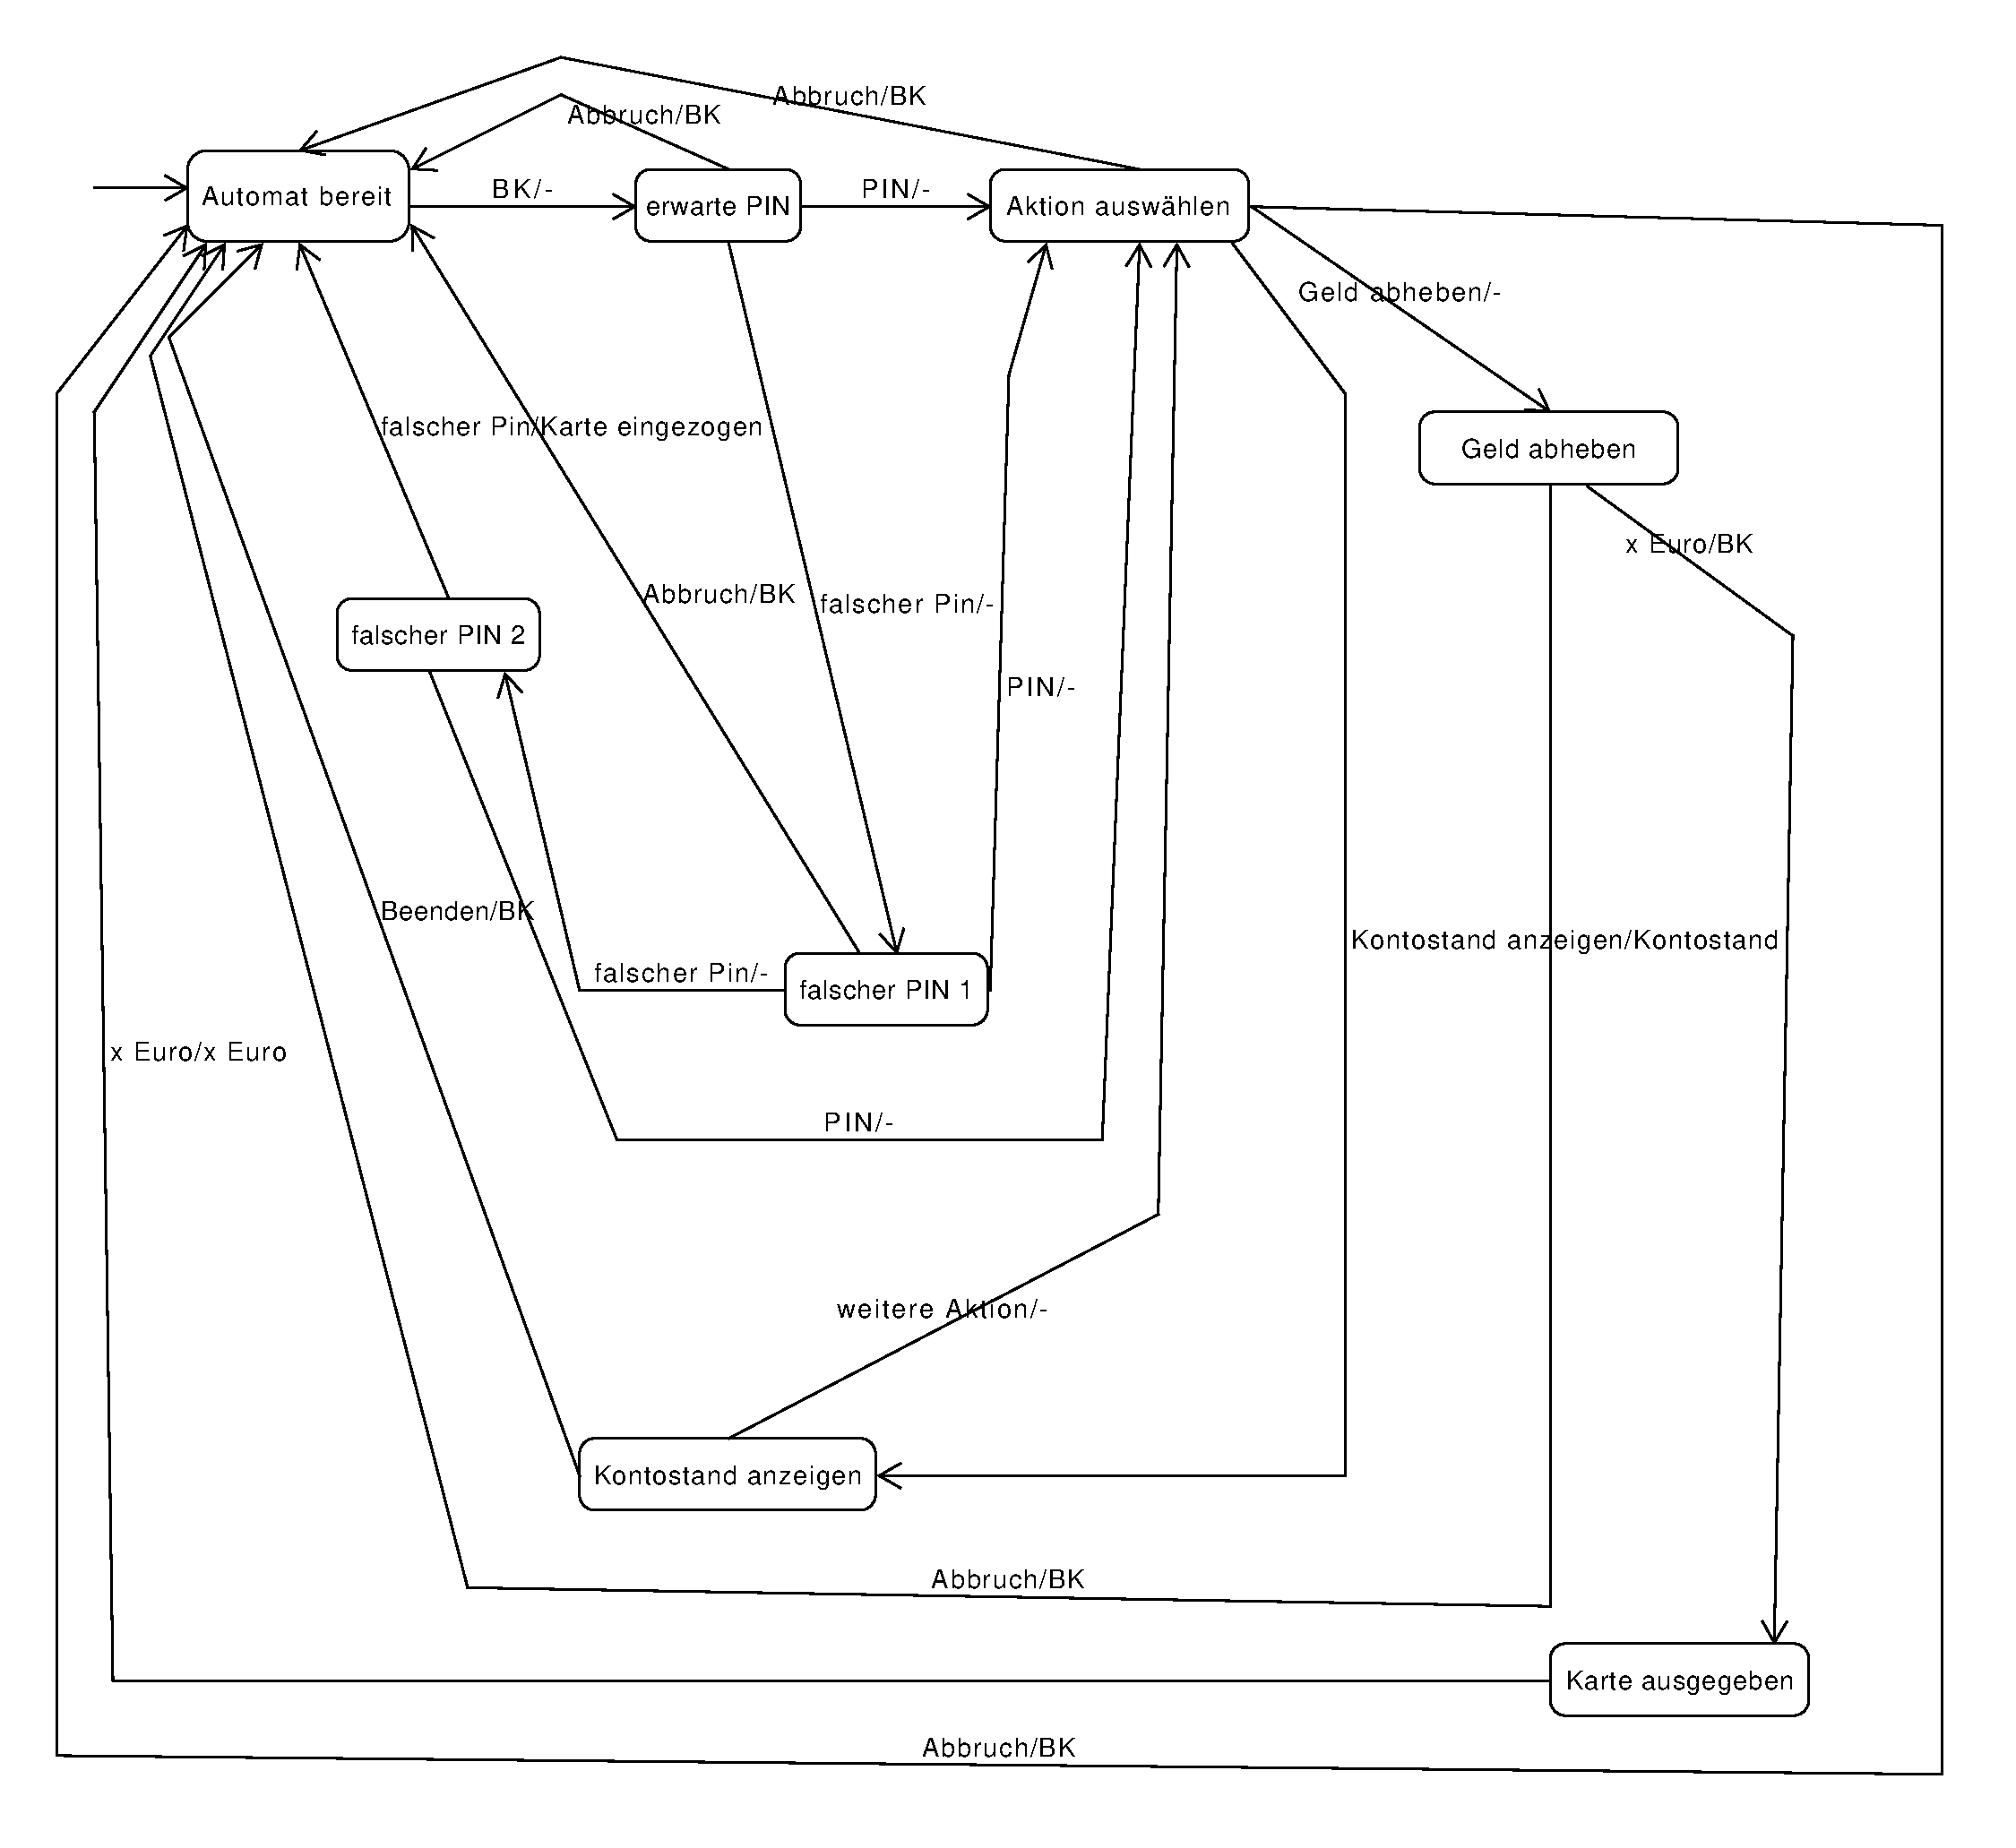
\includegraphics[width=\linewidth]{bankomat_v2.pdf}
\caption{Das UML-Zustandsdiagramm des Bankomaten.}
\end{center}
\end{figure}
	
\subsection{Code}

\subsubsection{Aufbau}

Der Automat wurde in einem header-only Modul Bankomat entwickelt. In der main-File wird eine Instanz des Automaten angelegt und per Kommando \begin{lstlisting}[language=c++]
sm.process_event()
\end{lstlisting} werden die Zustandsübergänge herbeigeführt.

\subsubsection{Zustände}

Wie man aus dem UML herauslesen kann, gibt es 8 verschiedene States, in denen sich der Automat befinden kann. Die Zustände werden erst im Transition Table definiert und verwendet. Siehe Codebeispiel Zustandsübergänge.

\subsubsection{Events}

Die Events führen immer zu einem Zustandsübergang, der manuell durch die Funktion \texttt{process\_event()} ausgelöst werden kann.

\begin{lstlisting}[language=c++]
struct karte_eingef{
};
struct pin{
};
struct abbruch{
};
struct geld_abheben_e{
};
struct kontostand_e{
};
struct x_euro{
};
struct weitere_aktion{
};
	
\end{lstlisting}
Sie werden einfach durch leere Strukturen definiert und in weiterer Folge von der State Machine verarbeitet.


\subsubsection{Zustandsübergänge - Transition Table}

Der Transition Table definiert aus welchem Ausgangszustand die State Machine durch welches Event in welchen Folgezustand wechselt. Hier wird auch der Startzustand durch einen * vor dem Namen definiert und die Guards und Actions werden bei den Zustandsübergängen aufgerufen.

\begin{lstlisting}[language=c++]
struct Automaton {

public:
  auto operator()() {
    return make_transition_table(
    
     *"automat_bereit"_s + event<karte_eingef> / []
     {} = "erwarte_pin"_s,
     
      "automat_bereit"_s + on_entry<_> / [] {
          std::cout << "Karte bitte!" << std::endl;
          std::cin >> karte;

          bool check_card{true};

          while(check_card){
                if(cards.find(karte) == cards.end()){
                std::cout << "Unguelitge Karte. Karte bitte!"
                << std::endl;
                std::cin >> karte;
            }
            else{
                karte_pin.pin = cards.at(karte);
                check_card=false;
            }
          }      
      },
      
      "erwarte_pin"_s + event<pin> [right_PIN] / []
      {} = "aktion_auswahlen"_s,
      
      "erwarte_pin"_s + event<abbruch> / []
      {} = "automat_bereit"_s,
      
      "erwarte_pin"_s + event<pin> [!right_PIN] / []
      {} = "falscher_pin1"_s,
      
      "erwarte_pin"_s + on_entry<_> / []
      {
          std::cout << "PIN eingeben!" << std::endl; 
          std::cin >> pin_;
          pin_inp.value = pin_;        
      },
      "falscher_pin1"_s + event<pin> [!right_PIN] / []
      {} = "falscher_pin2"_s,
      
      "falscher_pin1"_s + event<pin> [right_PIN] / []
      {} = "aktion_auswahlen"_s,
      
      "falscher_pin1"_s + on_entry<_> / [] {
          std::cout << "Fehler 1! PIN erneut eingeben!" << std::endl;
          std::cin >> pin_;
          pin_inp.value = pin_;
      },
      "falscher_pin2"_s + event<pin> [!right_PIN] / [] {
          std::cout << std::endl << "Karte eingezogen!" << std::endl;
          cards.erase(karte);
          } = "automat_bereit"_s,
    );
  }
};
	
\end{lstlisting}
Hier ein Ausschnitt aus dem Transition Table dieses Projektes. Der echte ist noch um einiges länger, dieser Teil soll nur zeigen, wie man sich diese Zustandsübergangstabelle vorstellen kann. Einige dieser Zeilen sind keine Definitionen für Übergänge, sondern beschreiben das Verhalten der State Machine beim Eintritt in verschiedene Zustände. Oft wird eine Eingabe erwartet und ein kurzer Text zur Orientierung ausgegeben.\newline\newline

Hier ein Beispiel für einen Zustandsübergang:

\begin{lstlisting}[language=c++]
*"automat_bereit"_s + event<karte_eingef> / []{} = "erwarte_pin"_s;
.
\end{lstlisting}
Und hier ein Beispiel für eine on\_entry-Aktion, die durchgeführt wird, sobald der Automat in diesen Zustand kommt:
\begin{lstlisting}[language=c++]
"automat_bereit"_s + on_entry<_> / [] {
          std::cout << "Karte bitte!" << std::endl;
          std::cin >> karte;

          bool check_card{true};

          while(check_card){
                if(cards.find(karte) == cards.end()){
                std::cout << "Unguelitge Karte. Karte bitte!"
                << std::endl;
                std::cin >> karte;
            }
            else{
                karte_pin.pin = cards.at(karte);
                check_card=false;
            }
          }      
      };
\end{lstlisting}

\subsubsection{Guards}

Guards sollen Zustandsübergänge mit falschen oder ungültigen Werten verhindern. Nur, wenn der guard \texttt{true} zurückliefert geht der Zustandsübergang durch.\newline\newline
Definition:
\begin{lstlisting}[language=c++]
const auto right_PIN = [](PIN& pin, Karte& karte){
    std::cout << "PIN VALUE:" << pin.value << std::endl;
    return pin.value == karte.pin;
};
\end{lstlisting}
Anwendung:

\begin{lstlisting}[language=c++]
"erwarte_pin"_s + event<pin> [right_PIN] / [] {} = "aktion_auswahlen"_s;
\end{lstlisting}
Dieser Guard vergleicht den eingegebenen (pin.value)
 mit dem richtigen, in der Liste eingatragenen PIN (karte.pin). Je nachdem, ob die beiden übereinstimmen, wird der Zustandsübergang zugelassen oder nicht.

\subsubsection{Login}

Um sich in den Bankomat einzuloggen, muss man zuerst seine Karte ''einlesen''. Das bedeutet, einfach entweder ''karte1'', ''karte2'' oder ''karte3'' eingeben, wenn man nach der Karte gefragt wird. Hat man diesen Schritt erfolgreich erledigt, wird man nach dem PIN gefragt. Der PIN für karte1 ist 1234, für karte2 6969 und für karte3 0420.

\subsubsection{Aktion auswählen}

In diesem Zustand wird der Benutzer gefragt, was er als nächstes machen will. Seine Möglichkeiten bestehen daraus, sich den Kontostand anzeigen zu lassen, Geld abzuheben oder den Vorgang abzubrechen und sich auszuloggen. Sollte er letzteres wählen, begibt sich der Automat wieder in den Startzustand und wartet au den Input einer Karte.

\subsubsection{Kontostand anzeigen}

Wählt der Benutzer die 2. Option Kontostand anzeigen aus, wird ihm der aktuelle Kontostand der Karte angezeigt, mit der er eingeloggt ist, bevor er automatisch wieder in den Zustand ''Aktion auswählen'' geleitet wird.

\subsubsection{Geld abheben}

Bei der ersten Auswahlmöglichkeit wird der User gefragt, wie viel Geld er abheben will. Hier ist des ihm nicht möglich, mehr als 400 Euro, oder in Minus hinein abzuheben. Sobald die Transaktion abgeschlossen ist und das Geld vom Konto abgezogen wurde, wird der Benutzer automatisch ausgeloggt und der Automat befindet sich wieder im Startzustand.

\end{spacing}
\end{document}




